\section{Introduction}

\paragraph{}The purpose of this lab was to get familiarized with many key tools and concepts that will be critical throughout this course. In order to gain a more practical understanding of how three phase power systems behave, we created a three phase circuit and performed two different experiments with it. These experiments showed us the effects of different types of loads on power. Specifically, the affect on real vs reactive power.

\section{Part 1: Effects of real and complex impedance on complex power and current.}
\paragraph{}The first part of the lab had us connect loads to the power source and read the voltage, current, frequency, real power, and reactive power under different types of loads using the data acquisition control interface. We first varied the load only by increasing the real resistance. Then we varied the load by changing the reactance and took measurements. We introduced both increasingly inductive and increasingly capacitive loads. The results are as follows.

\begin{figure}[H]
    \centering
        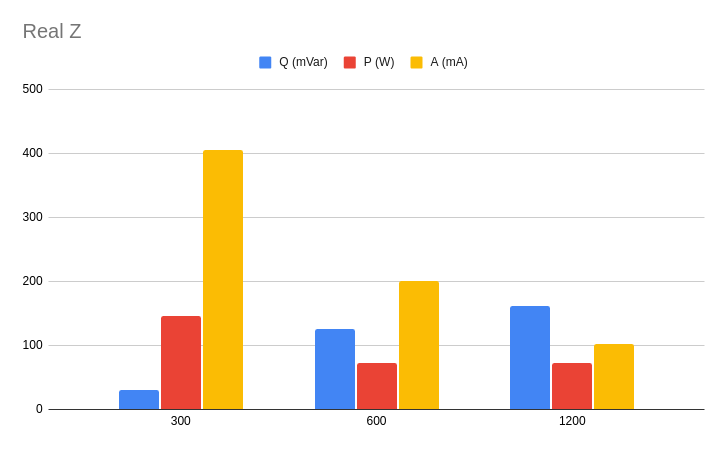
\includegraphics[angle=0, width=.65\linewidth]{real_z.png}
    \caption{\label{lab6drawing3.jpeg}Reactions to purely real impedance}
\end{figure}

\paragraph{} It is evident that as we increase the pure resistance of the load that the reactive power remains relatively constant, while the current and thus the real power drops significantly. While $Q$ does appear to increase slightly, it is on the order of milliamps, and is unlikely to be due to the increase in resistance.

\begin{figure}[H]
    \centering
        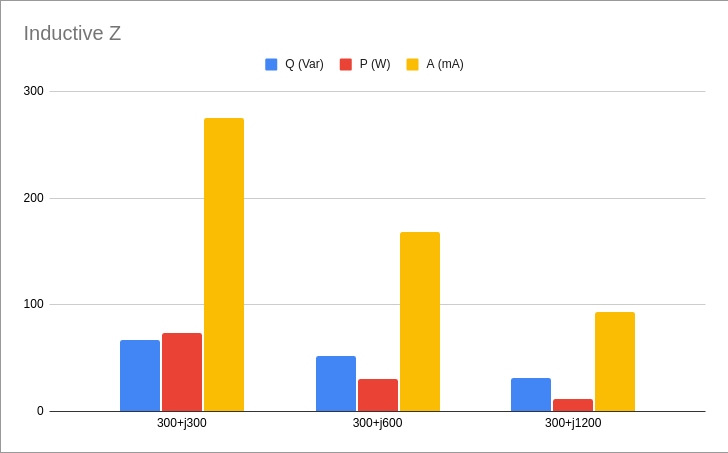
\includegraphics[angle=0, width=.65\linewidth]{ind_z.png}
    \caption{\label{lab6drawing3.jpeg}Reactions to purely inductive impedance}
\end{figure}

\paragraph{}Introducing an increasingly inductive load resulted in current dropping as $L$ increased. One interesting note is that $Q$ seemed to max out at $R = L$, and then fall as $L$ increased further. This is likely due to the relationship $Q = I^2X$, which shows that the rate of change of $Q$ is more dependent on $I$, which decreases as $|Z|$ increases, than it is on $X$. 

\begin{figure}[H]
    \centering
        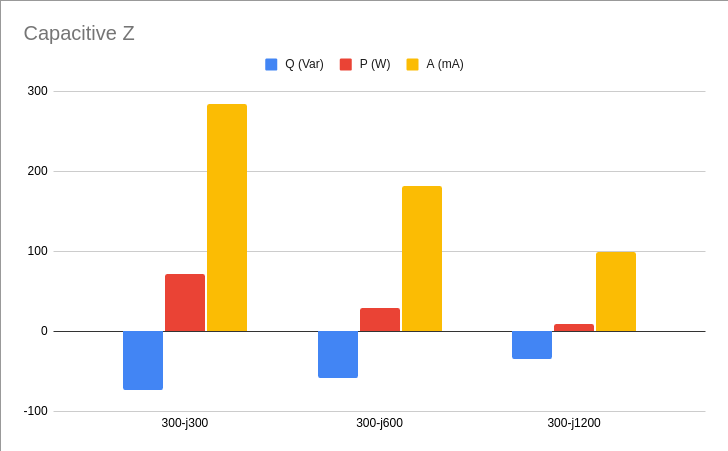
\includegraphics[angle=0, width=.65\linewidth]{cap_z.png}
    \caption{\label{lab6drawing3.jpeg}Reactions to capacitive impedance}
\end{figure}

\paragraph{} A similar behavior was observed when the we varied the capacitive load. The negative reactance topped out at $C = R$, and decreased as $C$ increased. The increased capacitance raised $|Z|$, which in turn lowered the current and therefore the magnitude of $Q$.

\section{Part 2: Effects of a mechanical load on power. }

\paragraph{}The second part of the lab involved connecting a three phase synchronous motor to the power source and using a dynamometer to apply mechanical load. Using the data acquisition control database, we measured voltage, current, frequency, real power, and reactive power under different DC excitation and mechanical loads. The first excitation level was set at 100 VDC to achieve zero reactive power with no mechanical load. We would then increase the mechanical torque and record the measurements. This would also be repeated for 90 VDC and 110 VDC excitation to observe how rotor excitation and mechanical loading would effect the motor's electrical behavior.  

\begin{figure}[H]
    \centering
        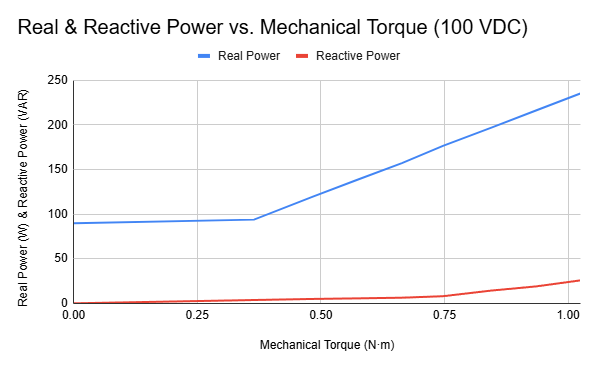
\includegraphics[angle=0, width=.65\linewidth]{100vdc.png}
    \caption{\label{lab6drawing3.jpeg}Result of mechanical torque on 100 VDC rotor excitation}
\end{figure}

\paragraph{}Starting with 100 VDC, as mechanical torque starts to increase the mechanical load on the motor, real power is used and gradually increases while reactive power starts at 0 VAR and slowly increases. This shows that minimal reactive power was being used at the start of the experiment, however as the mechanical load increased more reactive power was used from 0.75 N\textperiodcentered m to 1.00 N\textperiodcentered m.

\begin{figure}[H]
    \centering
        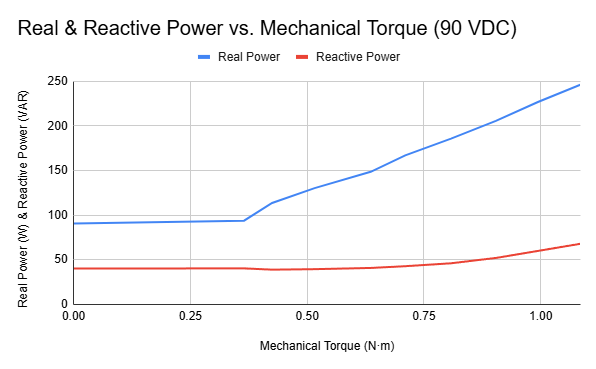
\includegraphics[angle=0, width=.65\linewidth]{90vdc.png}
    \caption{\label{lab6drawing3.jpeg}Result of mechanical torque on 90 VDC rotor excitation}
\end{figure}

\paragraph{}The excitation level was then dropped to 90 VDC. While Figure 5 shows real power still being consumed with a similar trend to the 100 VDC test, reactive power was also consumed at the start of mechanical loading and would increase as well. This shows that the motor was operating at a lower rotor excitation level and consumed reactive or inductive power from the power source.

\begin{figure}[H]
    \centering
        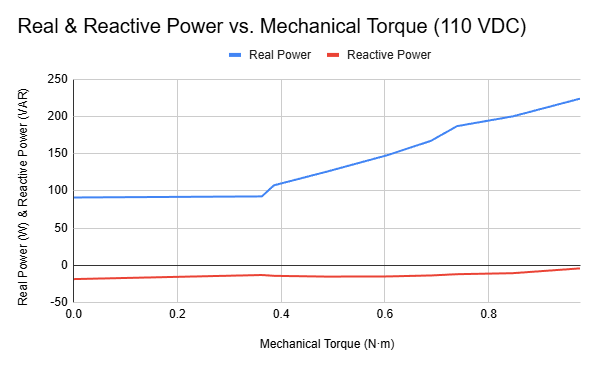
\includegraphics[angle=0, width=.65\linewidth]{110vdc.png}
    \caption{\label{lab6drawing3.jpeg}Result of mechanical torque on 110 VDC rotor excitation}
\end{figure}

\paragraph{}The excitation of the rotor was increased to 110 VDC. Although real power is still consumed at a similar rate as mechanical loading increased, reactive power would maintain a negative value. This indicated that the motor was behaving capacitively and supplying reactive power to the power source. As the mechanical loading increased the reactive power would approach 0 VAR, showing that the motor was supplying less reactive power with increased mechanical loading.

\section{Conclusion}
\paragraph{}Understanding the interplay between reactive loads, real power, and reactive power is distinctly important in the field of power engineering. Managing the power factor of a system is crucial to maintaining efficiency. This lab taught us to use many of the tools at our disposal in the power lab. It also clearly showed that tuning the value of the reactance either by varying the load, or applying a torque to a synchronous motor had a drastic effect on the amount of real power, as opposed to reactive power which is largely wasted, produced by the same voltage and nearly the same current. We also learned about the reactive power consumption characteristics of synchronous machines varying based on the applied DC voltage. Moving forward it will be exciting to learn more techniques to maximize efficiency, and deepen our understanding of the lab and the tools available to us. 